\documentclass{article}

\usepackage{booktabs}

\usepackage[utf8]{inputenc}

% Default fixed font does not support bold face
\DeclareFixedFont{\ttb}{T1}{txtt}{bx}{n}{12} % for bold
\DeclareFixedFont{\ttm}{T1}{txtt}{m}{n}{12}  % for normal

% Custom colors
\usepackage{color}
\definecolor{deepblue}{rgb}{0,0,0.5}
\definecolor{deepred}{rgb}{0.6,0,0}
\definecolor{deepgreen}{rgb}{0,0.5,0}

\usepackage{listings}

% Python style for highlighting
\newcommand\pythonstyle{\lstset{
language=Python,
basicstyle=\ttm,
morekeywords={self},              % Add keywords here
keywordstyle=\ttb\color{deepblue},
emph={MyClass,__init__},          % Custom highlighting
emphstyle=\ttb\color{deepred},    % Custom highlighting style
stringstyle=\color{deepgreen},
frame=tb,                         % Any extra options here
showstringspaces=false
}}


% Python environment
\lstnewenvironment{python}[1][]
{
\pythonstyle
\lstset{#1}
}
{}

\usetikzlibrary{automata,positioning}

%
% Basic Document Settings
%

\topmargin=-0.45in
\evensidemargin=0in
\oddsidemargin=0in
\textwidth=6.5in
\textheight=9.0in
\headsep=0.25in

\linespread{1.1}

\pagestyle{fancy}
\lhead{\hmwkAuthorName}
\chead{\hmwkClass\ (\hmwkClassInstructor\ \hmwkClassTime): \hmwkTitle}
\rhead{\firstxmark}
\lfoot{\lastxmark}
\cfoot{\thepage}

\renewcommand\headrulewidth{0.4pt}
\renewcommand\footrulewidth{0.4pt}

\setlength\parindent{0pt}

%
% Create Problem Sections
%

\newcommand{\enterProblemHeader}[1]{
    \nobreak\extramarks{}{Problem \arabic{#1} continued on next page\ldots}\nobreak{}
    \nobreak\extramarks{Problem \arabic{#1} (continued)}{Problem \arabic{#1} continued on next page\ldots}\nobreak{}
}

\newcommand{\exitProblemHeader}[1]{
    \nobreak\extramarks{Problem \arabic{#1} (continued)}{Problem \arabic{#1} continued on next page\ldots}\nobreak{}
    \stepcounter{#1}
    \nobreak\extramarks{Problem \arabic{#1}}{}\nobreak{}
}

\setcounter{secnumdepth}{0}
\newcounter{partCounter}
\newcounter{homeworkProblemCounter}
\setcounter{homeworkProblemCounter}{1}
\nobreak\extramarks{Problem \arabic{homeworkProblemCounter}}{}\nobreak{}

%
% Homework Problem Environment
%
% This environment takes an optional argument. When given, it will adjust the
% problem counter. This is useful for when the problems given for your
% assignment aren't sequential. See the last 3 problems of this template for an
% example.
%
\newenvironment{homeworkProblem}[1][-1]{
    \ifnum#1>0
        \setcounter{homeworkProblemCounter}{#1}
    \fi
    \section{Problem \arabic{homeworkProblemCounter}}
    \setcounter{partCounter}{1}
    \enterProblemHeader{homeworkProblemCounter}
}{
    \exitProblemHeader{homeworkProblemCounter}
}

%
% Homework Details
%   - Title
%   - Due date
%   - Class
%   - Section/Time
%   - Instructor
%   - Author
%

\newcommand{\hmwkTitle}{Assignment \ \#3}
\newcommand{\hmwkDueDate}{\today}
\newcommand{\hmwkClass}{Disrete Math}
\newcommand{\hmwkClassTime}{Section A}
\newcommand{\hmwkClassInstructor}{Professor J}
\newcommand{\hmwkAuthorName}{\textbf{V} \and \textbf{U}}

%
% Title Page
%

\title{
    \vspace{2in}
    \textmd{\textbf{\hmwkClass:\ \hmwkTitle}}\\
    \normalsize\vspace{0.1in}\small{Due\ on\ \hmwkDueDate\ at 3:10pm}\\
    \vspace{0.1in}\large{\textit{\hmwkClassInstructor\ \hmwkClassTime}}
    \vspace{3in}
}

\author{\hmwkAuthorName}
\date{}

\renewcommand{\part}[1]{\textbf{\large Part \Alph{partCounter}}\stepcounter{partCounter}\\}

%
% Various Helper Commands
%

% Useful for algorithms
\newcommand{\alg}[1]{\textsc{\bfseries \footnotesize #1}}

% For derivatives
\newcommand{\deriv}[1]{\frac{\mathrm{d}}{\mathrm{d}x} (#1)}

% For partial derivatives
\newcommand{\pderiv}[2]{\frac{\partial}{\partial #1} (#2)}

% Integral dx
\newcommand{\dx}{\mathrm{d}x}

% Alias for the Solution section header
\newcommand{\solution}{\textbf{\large Solution}}

% Probability commands: Expectation, Variance, Covariance, Bias
\newcommand{\E}{\mathrm{E}}
\newcommand{\Var}{\mathrm{Var}}
\newcommand{\Cov}{\mathrm{Cov}}
\newcommand{\Bias}{\mathrm{Bias}}

\begin{document}

\maketitle

\pagebreak
\begin{homeworkProblem}
    Let $G = (V,E)$ be a simple graph where $V$ is the set of vertices and $E$ is the set of edges.
    We denote the number of vertices by $n := |V|$ and the number of edges by $m := |E|$. 
    For a vertex $a \in V$ , we denote the degree of vertex $a$ by $d(a)$. Furthermore, denote the minimum degree of all vertex degrees by $\sigma$ and the maximum degree by $\delta$. 
    Please prove the statements below

    \textbf{(a)} The number of vertices that have odd degrees must be even;

    \textbf{(b)} $m \le \binom{n}{2}$

    \textbf{(c)} $\sigma \le \frac{2m}{n} \le \delta$

    \textbf{(d)} The length of a path is defined to be the number of edges in the path. Assume $n > 0$. Let $k \ge 0$ be an integer. If $\sigma \ge k$, then $G$ has a path with length $k$.

    \large \textbf{Solution.}

    \textbf{(a)}
    
    Recall the Handshake Theorem,
    \[\sum_{v\in V}d(v) = 2|E|\]
    The RHS is even, implying that the LHS is also even, thus $\#\{v\in V | d(v) \text{ is odd}\}$ must be even.
    
    \textbf{(b)}

    A simple fact is that $d(v) \le |V| - 1,\forall v\in V$, which means each vertex has at most $|V| - 1$ vertices to connect.
    Thus by Handshake theorem,

    \begin{align*}
        m = |E| &= \frac{\sum_{v\in V}d(v)}{2} \\
                &\le \frac{\sum_{v\in V} \left(|V| - 1\right)}{2} \\
                &= \frac{|V|(|V| - 1)}{2}\\
                &= \binom{|V|}{2}\\
                &= \binom{n}{2}
    \end{align*}

    \textbf{(c)}
    We calculate the average number of neibourhoods a vertex has, whcih is
    \[
        \frac{\sum_{v\ in V} d(v)}{|V|} = \frac{2 |E|}{|V|} = \frac{2m}{n}
    \]

    The average value should be larger than the minimum value whilst less than the maximum value. 
    Therefore
    \[\sigma \le \frac{2m}{n} \le \delta\]

    \textbf{(d)}

    We use mathematical induction on this one.

    If $k = 0$ it is trivial.

    If $k = 1$, since $\sigma \ge k$, a vertex called $v_0$ which $\sigma$ neibourhoods has at least one neibourhood, which is also a path with length $1$.

    Now assume that for $1 \le k < \sigma$, there is a path issuing from $v_0$, with a sequence of vertices $v_0v_1\cdots v_{k-1}$.

    Now we examine the situation of $v_{k-1}$. Let $D_{v_{k-1}}$ be the set of neibourhood of $v_{k-1}$. Clearly, $|D_{v_{k-1}}| = d(v_{k-1})\ge \sigma$.
    Now set $R = D_{v_{k-1}} - \{v | v\in {v_0, \cdots, v_{k-2}}\}$.

    Then $|R| \ge \sigma - (k-1) = \sigma - k + 1\ge 1$ Thus we can extend $v_0v_{k-1}$ by at least one edge so we have a path $v0\cdots v_k$ with length $k$.
    \qed


\end{homeworkProblem}
\begin{homeworkProblem}
    Let $G$ be a graph with $n - 1$ edges where $n$ is the number of vertices of $G$. 
    Show the following three statements are equivalent:

    (a) G is connected; (b) G has no cycles; (c) G is a tree.

    \textbf{Solution.}
    
    We first prove two lemmas.

    \subsection*{Lemma 1}

    A connected graph $G$ with $n$ and $n - 1$ edges removed by any edge is not connected.

    \textbf{proof.}

    If $n = 2$, there are two vertices, and one edge. Removing the only edge results in a two
    disconnected vertices.

    Assume that we have a connected graph with $k$ vertices and $k - 1$ edges. We now consider a connected
    graph with $|V| = k + 1$, and $|E| = k$
    
    Recall the Handshake Theorem,
    \[\sum_{v \in V}d(v) = 2 |E|\]

    Assume that $\forall v. d(v) \ge 2$, we have

    \[2k = 2 |E| = \sum_{v \in V}d(v) \ge \sum_{v\in V} 2 = 2 |V| = 2(k + 1)\]

    Which is $2k \ge 2k + 2$, a contradiction.

    Thus with the connectedness of $G$, $\exists v\in V. d(v) = 1$.
    We pick $v_0 \in V. d(v_0) = 1$.
    Remove $v_0$, and the edge that connects $v_0$.

    We then obtain a connected graph $G' = (V', E')$, with $|V'| = k, |E'| = k - 1$.
    According to the inductive hypothesis, Removing any edge of $G'$ results in a disconnected graph. 

    Now return $v_0$, and $v_0$'s edge back to $G'$, Now removing any edge
    of $G$, if it is the $v_0$'s edge, $G$ then is not connected, if it is other edge, then it
    is also disconnected, by the induction.
    \qed

    \subsection*{$(a) \implies (b)$}

    Assume the contrary, $G$ is connected and has a cycle.
    We remove one edge $e$ on any $G$'s cycle. On the one hand, since e is on the cycle, it does not affect the connectivity of $G$.

    On the other hand, by lemma 1, $G$ is not connected then. We have a contradiction.
    Therefore $(a) \implies (b)$.

    \qed

    \subsection*{$(b) \implies (c)$}

    Recall the definition of a Tree. A tree is a connected, and cycle-free graph.
    So we need to only show that $G$ is connected, if $G$ has no cycle.

    We again prove using induction. If there are two vertices and one edge, it has no cycle and connected for sure.
    Now assume any cycle-free graph $G$ with $k$ vertices and $k - 1$ edges is connected.

    Consider a cycle-free graph with $k + 1$ vertices and $k$ edges.
    Again it has a vertex $v_0$ $d(v_0) = 1$. Now hide $v_0$ along with its edge.
    We obtain a graph with $|V| = k$, $|E| = k - 1$.

    By induction, it is also cycle-free and thus connected. 
    Add $v_0$ and its edge back we conclude that $G$ is also connected.
    \qed.

    \subsection*{$(c) \implies (a)$}
    
    The definition of Tree tells us that a tree is connected.
    \qed
\end{homeworkProblem}

\begin{homeworkProblem}
    A walk in a graph $G$ is a sequence $W := v_0e_1v_1 ...v_{l-1}e_lv_l$, whose terms are alternately vertices and edges of $G$ (not necessarily distinct), such that $v_i-1$ and $v_i$ are the ends of $e_i,1 \le i \le l$.
A closed walk is a walk that starts from and ends on the same vertex. So an Eulerian cycle is a closed walk that traversed each edge exactly once and we also call it Eulerian tour.
(Be cautious that an Eulerian cycle is not a cycle. Recall that, by definition, a cycle should be a connected (sub)graph whose vertices are all of degree $2$.)
We say that a graph is Eulerian if it contains an Eulerian tour. So we know an Eulerian graph has no vertices of odd degree. Let $G$ be Eulerian.

\textbf{(a)} Prove that G contains a cycle;

\textbf{(b)} For two cycles with no edges in common, we call they are edgedisjoint. 
Please show that the edge set of $G$ can be partitioned into edge sets corresponding to edge-disjoint cycles in the graph.

\textbf{Solution for (a).}

First off we note that $G$ is connected. If it has no cycle, then it is a tree.
Apparently, we can't traverse each edge only once and get back to the starting point in a tree.
\qed

\textbf{Solution for (b).}

First off, we prove a lemma: for any $v \in v. d(v)$ is even.
Assume $v0$ is the starting point of a Eulerian tour. To commence a
Eulerian tour, one must leave $v$ and then come back to $v$ repeatly. Thus $v$ needs
even number of neibourhood to achieve this goal, otherwise the Eulerian tour will never end at $v$.
Same for other vertex $w$, one must come into $w$ and then finally will leave. Without $d(w)$ being even, the Eulerian tour will finally end at $w$ which
is impossible. \qed

Now let $C_0$ be a cycle of $G$. Removing $C_0$ from $G$ we obtain $G_0$ which has every vertex $v$, $d(v)$ is even since a cycle is of degree $2$ for each vertex.
Repeating this process, removing any cycle $C_k$ from $G_{k - 1}$ obtaining $G_k$. The invariant is that $d(v)$ is even for any vertex in $G_{k - 1}$.
If there is a $k$ for which $G_k$ ends up having a connected component being a tree which doesn't have a cycle, then in this tree there is a vertex whose degree is one, an odd number. This is a contradiction.  
\qed 

\end{homeworkProblem}

\begin{homeworkProblem}
    A k-regular graph is a graph in which every vertex is of degree $k$. The girth of a graph is the length of the shortest cycle of the graph. Prove that

    (a) A k-regular graph of girth four has at least $2k$ vertices;

    (b) A k-regular graph of girth five has at least $k^2 + 1$ vertices.

    \textbf{Solution for (a)}

    Pick $v_0 \in V$. Let $N_{v_0} = \{v_1, v_2, \cdots , v_k\}$ be the set of neibourhood of $v_0$.
    Since there is no triangle in $G$ with all $3$ edges in $E$, for any $i, j$ in $\{1,\cdots,k\}$, $\{v_i, v_j\}\not \in E$
    $\forall w \in N_{v_j} - \{v_0\}, {w, v_0} \not \in E$. 
    Let $N'_{v_i} := N_{v_i} - {v_0}$, then $|N'_{v_i}| = 1$.

    Thus 
    \begin{align*}
        |V| &\ge \left|\{v_0\} \bigcup N_{v_0} \bigcup \left(N'_{v_1}\cup\cdots\cup N'_{v_k}\right)\right| \\
            &= 1 + k + |\left(N'_{v_1}\cup\cdots\cup N'_{v_k}\right)|\\
            &\ge 1 + k + |N'_{v_i}| \\ 
            &= 1 + k + k - 1 \\
            &= 2k
    \end{align*}

    \textbf{Solution for (b)}

    Pick $v_0, w_0 \in V$, such that $\{v_0, w_0\} \in E$, and set $w_k = v_0, v_k = w_0$. Because there is no triangle in $G$,
    $N_{v_0} \cap N_{w_0} = \{\}$. Let $N_{v_0} = \{v_1, v_2, \cdots , v_k\}, N_{w_0} = \{w_1, \cdots, w_k\}$ Let $N_v := \bigcup_{i = 1}^{k - 1} (N_{v_i} - \{v_0\}), N_w :=  \bigcup_{i = 1}^{k - 1} (N_{w_i} - \{w_0\})$
    We have $N_v \cap N_w = \{\}$ otherwise there will be a quadrilateral $\{v_0, v_i, w_j, w_0\}$ for some $1\le i, j\le k$. For the same reason, $N_{v_i}\cap N_{v_j} = \{\}$, and $N_{w_i}\cap N_{w_j} = \{\}, \forall 1\le i, j \le k$.
    Hence \[|N_v| = |N_w| = \sum_{s=1}^{k-1}(k-1) = (k-1)^2\]

    Thus
    \begin{align*}
        |V| &\ge \left|\{v_0, w_0\}\bigcup \left(N_{v_0} - \{w_0\}\right)\cup \left(N_{w_0} - \{v_0\}\right)\bigcup (N_v \cup N_w)\right|\\
            &= 2 + (k - 1) + (k - 1) + |N_{v} \cup N_{w}| \\
            &\ge 2 + (k - 1) + (k - 1) + |N_{v}| \\ 
            &=2 + 2(k - 1) + (k - 1)^2 \\ 
            &= 1 + (k - 1 + 1)^2 \\
            &= k^2 + 1
    \end{align*}
    \qed
    
\end{homeworkProblem}

\pagebreak

\begin{homeworkProblem}

    Please use Gale-Shapley’s algorithm to find one stable matching for thepreference lists below.


    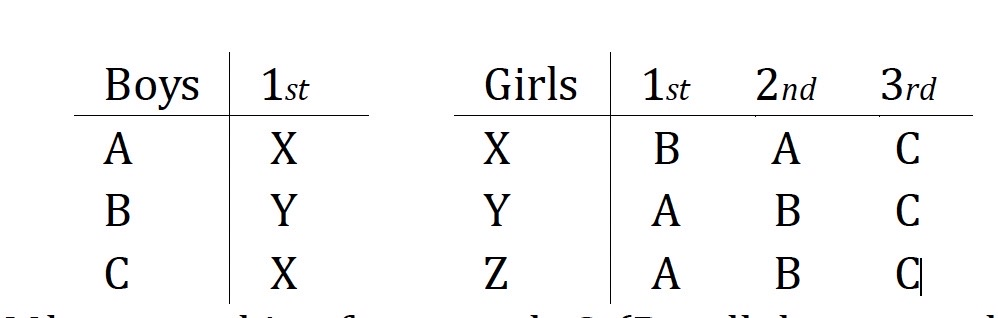
\includegraphics[scale=0.5]{./table.jpeg}

    \textbf{Solution}.

    We first consider boy $A$, Girl $X$ is on his top of list, then match $(A, X)$.
    Next Step consider Boy $B$. $Y$ is on his top of list and not ye purposed, then match $(B, Y)$.
    Now consider boy $C$. $X$ is on the top of his list, yet $X$ is matched with $A$. So we can't change anything here. 
    Next we consider $Y$, $Y$ is already matched with $B$ and $Y$ rank $B$ over $C$. Thus no change here as well.
    Therefore, the only choice of $C$ is $Z$
\end{homeworkProblem}

\begin{homeworkProblem}
    Let $M$ be a matching for a graph $G$. (Recall that a matching in a graph is a set of edges that do not have common vertices.)
    An alternating path is a path that begins with an unmatched vertex and whose edges belong alternately to the matching $M$ and not to the matching.
    An $M$-augmenting path is an alternating path that starts from and ends on unmatched vertices.
    Show that $M$ is a maximum matching if and only if $G$ has no $M$-augmenting path.

    \textbf{Proof of Necessity}

    Assume the contrary that $G$ has a $M$-augmenting path 
    \[P:=v_0 \xrightarrow{m_0} v_1 \xrightarrow{m_1} v_2\xrightarrow{m_2}\cdots\xrightarrow{m_k} v_{k+1}\]
    where $m_{2i + 1} \in M$
    On the other hand, let $M\bigoplus P := (M \cup P) - (M \cap P)$ denote the symmetric difference. We'll show that $M\bigoplus P$ is also a match and $\left|M\bigoplus P\right| = |M| + 1$.
    After action of the symmetric difference, edges in $M$ not in $P$ stay invariant, while all $m_i$ with even subscription remains,
    which are not in $M$, and the number of which exceeds the number of $m_j$ who are in $M$ by exactly one(since $k + 2$ is odd).
    Thus $\left|M\bigoplus P\right| = |M| + 1$ which contradicts to the maximality of $M$.
    \qed

    \textbf{Proof of Sufficiency}

    Assume that the largest matching is not $M$ but $M'$. Let $S := M \bigoplus M'$. We'll show that $P$ contains a $M'$-augmenting path.
    First off, we compare the number of element of $M$ in $S$, and the number of $M$ in $S$, which
    are $m := |M| - |M\cap M'|$ and $m' := |M'| - |M\cap M'|$ respectively. clearly $m' > m$. 
    Let $P$ be a path in $S$. Its edges must be alternative between $M$ and $M'$ and in this case the number of edge in $M'$ should be equal to the number
    of edge in $M'$. Otherwise it is a $M'$-augmenting path or $M$-augmenting path; it would lead to a contradiction. Since $m' > m$, some paths in $S$ must be $M$-augmenting which is also a contradiction.
    \qed 

\end{homeworkProblem}


\end{document}